\section{Ejercicio 2: Introducci\'on al dise\~no de filtros}
En esta secci\'on se propone el dise\~no de cuatro filtros de segundo orden, cada uno de un diferente tipo,
ya sea un pasabajo, pasaalto, pasabanda y rechazabanda. El objetivo de tal dise\~no es encontrar una funci\'on matem\'atica
que desde un punto de viste te\'orico modele o describa a los filtros, y luego analizar su implementaci\'on a trav\'es del uso de lo que se
denomina un Gyrator, lo cual ser\'a abordado y explicado posteriormente. Se establecen como criterios de dise\~no para los filtros la siguiente tabla:

\begin{table}[H]
    \centering
    \begin{tabular}{c c c c}
        Tipo de filtro & $f_p [Hz]$ & $f_a [Hz]$ & $f_c [Hz]$ \\
        \hline \\
        Pasabajos & $3kHz$ & $10.5kHz$ & $-$ \\
        Pasaaltos & $3.5kHz$ & $1kHz$ & $-$ \\
        Pasabanda & $-$ & $-$ & $6kHz$ \\
        Rechazabanda & $-$ & $-$ & $1kHz$ \\
        \hline
    \end{tabular}
    \caption{Condiciones de dise\~no}
\end{table}

En el caso del filtro pasabajos, se requiere que para frecuencias $f < f_p$ la ganancia sea superior a los $-3dB$ y que para frecuencias donde $f > f_a$ la ganancia
sea menor que $-10dB$. Por otro lado, para el caso del filtro pasaaltos, se requiere que para $f < f_a$ la ganancia sea menor que $-10dB$ y para $f > f_p$ la ganancia
sea mayor que $-3dB$.

Habiendo obtenido los desarrollos te\'oricos para fundamentar las implementaciones de cada uno de los circuitos requeridos, se los simular\'a e
implementar\'a pr\'acticamente, para poder contrastar los comportamientos en estos diferentes contextos, con el fin de evaluar el resultado obtenido.

\subsection{Introducci\'on Te\'orica}
El objetivo de esta introducci\'on te\'orica es presentar de forma breve y sencilla una serie de conceptos que puede ser considerados fundamentales
para comprender el an\'alisis realizado posteriormente a lo largo del desarrollo.

\subsubsection{Filtros de segundo orden}
Para los prop\'ositos del desarrollo a realizar, se entiende un filtro como un sistema descripto por una funci\'on transferencia $H(s)$ que se asume lineal, de tiempo invariante
y bibo-estable, tal que su respuesta en frecuencia $H(f)$ modula en amplitud y fase las se\~nales de entrada, produciendo efectos diferenciados seg\'un la frecuencia de las mismas. Por ende,
se puede realizar una clasificaci\'on de tipos de filtros seg\'un la forma en la cual la respuesta en frecuencia del sistema modula las se\~nales de entrada. Usualmente para describir a los filtros se toman
frecuencias cr\'iticas o de referencia denominadas frecuencias de corte.

\begin{itemize}
    \item Filtros pasabajos: Aten\'uan \'unicamente para frecuencias superiores a la frecuencia de corte.
    \item Filtros pasaaltos: Aten\'uan \'unicamente para frecuencias inferiores a la frecuencia de corte.
    \item Filtros pasabanda: Aten\'uan todas las frecuencias exceptuando un rango de frecuencias en torno a la frecuencia de corte.
    \item Filtros rechazabanda: Aten\'uan para un rango de frecuencias en torno a la frecuencia de corte.
\end{itemize}

Luego, dado que el filtro se ve descripto por una funci\'on transferencia $H(s)$ podemos caracterizarlo seg\'un su orden, de ah\'i que en este desarrollo se emplear\'an sistemas de segundo orden.
Adem\'as, los filtros en su implementaci\'on pueden ser de car\'acter pasivos o activos seg\'un los componentes que lo integren y su comportamiento en t\'erminos energ\'eticos, particularmente cuando se emplean
amplificadores operacionales, usualmente se trabaja con un filtro activo, como ser\'a el caso de este trabajo.

\subsubsection{Gyrator}

\begin{figure}[H]
    \centering
    \includegraphics[scale=0.7]{../EJ2/Recursos/gyrator.png}
    \caption{Modelo del Gyrator}
    \label{fig:gyrator_modelo}
\end{figure}

El Gyrator es un dispositivo que inicialmente surgi\'o como un modelo te\'orico caracterizado por ser un cuadripolo no rec\'iproco con par\'ametros de impedancia
descriptos como se muestra en la expresi\'on de la Ec. \ref{eq:parametros_gyrator}. La funci\'on principal de un Gyrator es la de girar o invertir una impedancia, permitiendo
de esta forma simular la presencia de componentes inductivos a partir de componentes capacitivos, lo cual era buscado ya que la implementaci\'on real de un inductor a trav\'es de una bobina
no tiene un buen rendimiento para bajas frecuencias, suelen ser elementos grandes y funcionan bien para una frecuencia particular de construcci\'on.

\begin{equation*}
    \begin{pmatrix}
        V_1 \\ V_2
    \end{pmatrix}
    =
    \begin{pmatrix}
        0 & -r \\
        r & 0
    \end{pmatrix}
    \cdot 
    \begin{pmatrix}
        I_1 \\ -I_2
    \end{pmatrix}
    \label{eq:parametros_gyrator}
\end{equation*}

En la pr\'actica resulta necesario implementar circuitos de segundo orden para construir filtros, para lo cual las configuraciones m\'as usuales son circuitos
t\'ipicos RLC, no obstante para dichos casos se necesitar\'ia utilizar inductores que presentan una serie de desventajas que pueden ser sobrellevadas si se los reemplaza para ello un circuito Gyrator.
De esta forma, se logra invertir la impedancia de un capacitor para agregar al circuito una componente inductiva que le de el car\'acter de segundo orden al sistema, y para ello existen una gran diversidad
de circuitos que permiten implementar al Gyrator. En la Fig. \ref{fig:circuito_gyrator} se muestra una de ellas utilizando \'unicamente un s\'olo amplificador operacional.

\begin{figure}[H]
    \centering
    \includegraphics[scale=0.6]{../EJ2/Recursos/circuito_gyrator.png}
    \caption{Circuito Gyrator con un amplificador operacional}
    \label{fig:circuito_gyrator}
\end{figure}

Con el objetivo de comprender en detalle el funcionamiento de este circuito, se realizar\'an diversos an\'alisis ya sean cuantitativos o cualitativos que permitan
obtener conclusiones sobre la operaci\'on del circuito y c\'omo debe ser usado en la pr\'actica para lograr realizar el armado de filtros que requieren una componente inductiva.

\paragraph*{An\'alisis circuital: } Desde un punto de vista circuital, analizando al circuito como un cuadripolo al cual se busca la impedancia de entrada $Z_{IN} = \frac{V_{IN}}{I_{IN}}$.
Para realizar este desarrollo se considera inicialmente un amplificador operacional ideal en una configuraci\'on conocida como seguidor de tensi\'on o buffer, es sabido que un an\'alisis desde tal punto de vista
dar\'a una idea del funcionamiento del circuito, mientras que los modelos m\'as reales de tal amplificador operacional determinar\'an para qu\'e rangos de operaci\'on son v\'alidos tales resultados.

\begin{eqnarray*}
    I_{IN} & = I_L + I_C \\
    I_C & = \frac{V_{IN}}{R_C + \frac{1}{s \cdot C}} \\
    I_L & = \frac{V_{IN}}{R_L} \cdot \frac{1}{1 + s \cdot C \cdot R}
\end{eqnarray*}

\begin{equation}
    Z_{IN} = \frac{V_{IN}}{I_{IN}} = \frac{R_L + s \cdot C \cdot R_C \cdot R_L}{1 + s \cdot C \cdot R_L}
\end{equation}

Resulta interesante que tal circuito tiene una representaci\'on equivalente que puede ser demostrada llegando en ambos casos a la misma impedancia de entrada,
desde un punto de vista ideal puede ser empleado tal modelo equivalente para el dise\~no de los circuitos deseados, y determinar en qu\'e rangos de operaci\'on los resultados
son v\'alidos. En la Fig. \ref{fig:equivalente_gyrator} se ilustra tal modelo equivalente para el circuito propuesto.

\begin{figure}[H]
    \centering
    \includegraphics[scale=0.6]{../EJ2/Recursos/equivalente_gyrator.png}
    \caption{Circuito equivalente para el Gyrator con un opamp}
    \label{fig:equivalente_gyrator}
\end{figure}

\begin{equation}
    Z_{IN} = \frac{V_{IN}}{I_{IN}} = (s \cdot C \cdot R_C \cdot R_L + R_L) // (\frac{1 + s \cdot R_C \cdot C}{s \cdot C})
    \Rightarrow Z_{IN} = \frac{R_L \cdot (1 + s \cdot C \cdot R_C)}{1 + s \cdot C \cdot R_L}
\end{equation}

En una primera instancia, el an\'alisis que podr\'ia realizarse de este circuito es que si se considera una dada frecuencia de corte 
$\omega_o = \frac{1}{C \cdot R_L}$, luego puede establecerse que para frecuencias que cumplan ser $\omega << \omega_o \Rightarrow \frac{\omega}{\omega_o} << 1$ y bajo esta consideraci\'on
ser\'ia posible caracterizar al circuito como una bobina, donde la impedancia de entrada se puede aproximar como $Z_{IN} = R_L + s \cdot C \cdot R_C \cdot R_L$. Este an\'alisis final busca
intentar ver en el Gyrator condiciones para las cuales pueda ser pensado como lo que dio inicio a la b\'usqueda de este circuito, que es la simulaci\'on de un inductor, m\'as all\'a de que con la aproximaci\'on tomada
el resultado haya sido una bobina de inductancia equivalente $L = C \cdot R_C \cdot R_L$ y factor de calidad $Q = \omega \cdot R_C \cdot C$.

\paragraph*{An\'alisis del circuito realimentado:} si bien pudieron obtenerse resultados concretos del an\'alisis circuital del Gyrator propuesto, resulta de inter\'es buscar otros enfoques
para obtener una mayor comprensi\'on del funcionamiento de este circuito. Con esto en mente, se propone establecer un an\'alisis cualitativo del funcionamiento y luego describirlo empleando
la teor\'ia de sistemas realimentados.

En un principio, si se observa nuevamente el circuito de la Fig. \ref{fig:circuito_gyrator} e imaginariamente se desconecta el buffer y la resistencia $R_L$, lo que se tiene es un circuito simple RC,
no obstante al agregar la otra parte de la configuraci\'on se crea una realimentaci\'on positiva dentro del circuito. Consid\'erese este sistema donde inicialmente s\'olo se posee la rama RC la cual fija una corriente correspondiente, luego cuando
se conecta el lazo, el mismo sensa la tensi\'on de la resistencia $R_C$ lo cual equivale indirectamente a sensar la corriente en dicha rama, e inyecta una corriente proporcional en contrafase en la entrada. Esto \'ultimo produce constamente un desplazamiento de la corriente
total desde el $1^{\circ}$ al $4^{\circ}$ cuadrante. Esto mismo se puede observar en el diagrama fasorial con valores arbitrarios de la Fig. \ref{fig:fasores_gyrator}.

\begin{figure}[H]
    \centering
    \includegraphics[scale=0.8]{../EJ2/Recursos/fasores_gyrator.png}
    \caption{Diagrama fasorial para caracterizar la inversi\'on de impedancia del Gyrator}
    \label{fig:fasores_gyrator}
\end{figure}

Luego pasando a un an\'alisis m\'as cuantitativo del sistema realimentado, consid\'erese al sistema caracterizado por su impedancia de entrada, para lo cual se modeliza al mismo con entrada de corriente $I_{IN}$ y salida en $V_{IN}$,
entonces partiendo de las ecuaciones ya empleadas en el an\'alisis circuital, se puede considerar el siguiente diagrama en bloques del sistema a lazo cerrado, ilustrado en la Fig. \ref{fig:sistema_gyrator}.

\begin{figure}[H]
    \centering
    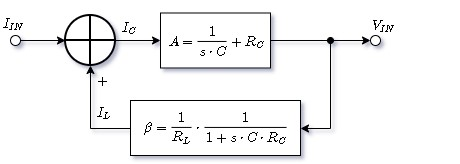
\includegraphics[scale=0.7]{../EJ2/Recursos/sistema_gyrator.jpg}
    \caption{Sistema a lazo cerrado del circuito Gyrator propuesto}
    \label{fig:sistema_gyrator}
\end{figure}

Se caracteriza la funci\'on transferencia, es decir la impedancia de entrada del circuito, en t\'erminos generales se llega a que:

\begin{equation}
    Z_{IN}(s) = \frac{A}{1 - \beta \cdot A}
\end{equation}

Particularmente para los casos donde, como suele suceder con los sistemas a lazo cerrado, la magnitud de $A >> 1$, entonces se puede aproximar
la funci\'on como:

\begin{equation}
    Z_{IN}(s) \approx \frac{1}{\beta} = R_L + s \cdot C \cdot R_C \cdot R_L
\end{equation}

Desde este punto de vista, para tales condiciones el circuito se comporta como una bobina, lo cual coincide con el an\'alisis puramente circuital.

\subsection{Filtro Pasabajos}

\subsubsection{Dise\~no de funci\'on transferencia}


\subsubsection{Dise\~no de circuito con Gyrator}
\subsubsection{Rangos de operaci\'on}
\subsubsection{Resultados}

\subsection{Filtro Pasaaltos}
\subsubsection{Dise\~no de funci\'on transferencia}
\subsubsection{Dise\~no de circuito con Gyrator}
\subsubsection{Rangos de operaci\'on}
\subsubsection{Resultados}

\subsection{Filtro Pasabanda}
\subsubsection{Dise\~no de funci\'on transferencia}
\subsubsection{Dise\~no de circuito con Gyrator}
\subsubsection{Rangos de operaci\'on}
\subsubsection{Resultados}

\subsection{Filtro Rechazabanda}
\subsubsection{Dise\~no de funci\'on transferencia}
\subsubsection{Dise\~no de circuito con Gyrator}
\subsubsection{Rangos de operaci\'on}
\subsubsection{Resultados}

\subsection{Implementaci\'on pr\'actica}
